% Texcount ignores the longtables
%TC:group longtable 0 0

\chapter{Testing and evaluation}\label{ch:testing-and-evaluation}
Using the implemented solution from Chapter~\ref{ch:implementation-of-the-solution} to test and evaluate its
effectiveness, both functional unit tests and agent training evaluation have been designed. To confirm that the
environment and agents implemented in the previous chapter
(section~\ref{sec:implementing-auction-and-resource-allocation-agents}) works as intended, unit testing has been added
that is explained in Section~\ref{sec:functional-testing}. While to evaluate the effectiveness of the proposed
solution from Section~\ref{sec:proposed-agents}, a range of metric have been measured during training in order to
test and compare implemented agents, neural network architectures and training parameters. These results are explained
in Section~\ref{sec:agent-evaluation}.

\section{Functional testing}\label{sec:functional-testing}
To confirm that the implementation of the agents and environment correctly, PyTest a module within python has been used
to design functions are valid. These tests are split into three families: agent, environment and training that are
explained in the respective tables~\ref{tab:agent_testing},~\ref{tab:env_testing} and~\ref{tab:training_testing}.
The results from the testing is shown in figure~\ref{fig:pytest_results}.

\begin{longtable}{|p{3cm}|p{11cm}|} \hline
    \textbf{Testing name} & \textbf{Explanation} \\ \hline
    Building agents & Constructs all of the agents with possible arguments to confirm agents can accept of all its
        attributes\\ \hline
    Saving agents & Confirms that agents can successfully save their neural networks and can successfully load
        the network again and is equal to the agent network. \\ \hline
    Agent actions & Confirms that all agents can generate valid actions for both bidding and weighting \\ \hline
    Gin config file & Gin is used to set the arguments used during training, to confirm that the file is valid. \\ \hline
    Building networks & Constructs all of the neural networks to confirm that the network return a valid output. \\ \hline
    Agent epsilon policy & While training, some of the agent actions are randomly selected to train the agents over
        a large area of the state. This tests that the random actions selected are valid. \\ \hline
    \caption{Table of testing functions for the agent}
    \label{tab:agent_testing}
\end{longtable}

\begin{longtable}{|p{3cm}|p{11cm}|} \hline
    \textbf{Testing name} & \textbf{Explanation} \\ \hline
    Saving and loading an environment & The environment allows for the saving the environment at its current
        state. This tests that the environment can save and reload the environment successfully. \\ \hline
    Loading environment settings & Tests that the load environment settings correctly generates a new random
        environment based on the settings. \\ \hline
    Random action environment steps & To tests that inputs to the auction and resource allocation steps are valid,
        random actions are generated for the environment, that is repeated for the whole environment.  \\ \hline
    Auction step & To confirm the Vickrey auction mechanism is completely implemented, a range of possible inputs
        are tested to confirm that right price and server the task is allocated to. \\ \hline
    Resource allocation step & To confirm that servers allocate their resources correct given some inputs. \\ \hline
    Allocation of computational resources & Checks that the server correctly allocates computational resources to
        allocated tasks. \\ \hline
    Allocation of storage and bandwidth resources & Checks that the server correctly allocates storage and
        bandwidth resources to allocated tasks. \\ \hline
    Allocation of all resources & Checks that resources are allocated by the server correctly for all of the
        resources. \\ \hline
    \caption{Table of testing functions for the environment}
    \label{tab:env_testing}
\end{longtable}

\begin{longtable}{|p{3cm}|p{11cm}|} \hline
    \textbf{Testing name} & \textbf{Explanation} \\ \hline
    Task pricing training & Tests that the task pricing reinforcement learning agents can correctly learning from
        different auction observations. \\ \hline
    Resource allocation training & Tests that resource allocation reinforcement learning agents can correctly
        learning from different resource allocation observations. \\ \hline
    Agent evaluation & Tests that the agent evaluation function for during training correctly captures the correct
        information due to the actions taken. \\ \hline
    Agent training & Tests that agents can be correctly trained over an environment with different actions and
        observations. \\ \hline
    Random actions training & Tests that agents with random actions that can quickly using the environment training
        methods to confirm that the function work as intended. \\ \hline
    \caption{Table of testing functions for agent training}
    \label{tab:training_testing}
\end{longtable}

\begin{figure}[h]
    \centering
    \includegraphics{figures/4_testing_eval_figs/pytest_results.PNG}
    \caption{Results of the unit functions described in the Tables~\ref{tab:agent_testing},~\ref{tab:env_testing}
        and~\ref{tab:training_testing}}
    \label{fig:pytest_results}
\end{figure}

\section{Agent evaluation}\label{sec:agent-evaluation}
In order to compare the implemented agents from Chapter~\ref{ch:implementation-of-the-solution}, a range of metric are
used which are recorded while the agent is training. For the auction agent the metrics are: histogram winning prices,
number of no bids, number of failed tasks, number of completed tasks and a histogram of actions taken. For the resource
allocation agents the metrics are a histogram of weighting, number of failed tasks and number of completed tasks.
Using these metrics evaluation of agent performance can be done between the different reinforcement learning algorithms
implemented in Table~\ref{tab:reinforcement_learning_algorithms}, network architectures in
Table~\ref{tab:neural_network_layers} and methods of training different agents. \\
These evaluations fall into three families: env and agent num, algorithm and network architecture that are analysed in
Subsections~\ref{subsec:environment-and-agent-number-training},~\ref{subsec:reinforcement-learning-algorithm-training}
and~\ref{subsec:neural-network-architecture-training} respectively.

\subsection{Environment and Agent number training}\label{subsec:environment-and-agent-number-training}
%% Single env
%% Multi env
%% Comparison on single env testing and multiple env and new environments
There are huge ranges of possible environment settings that agents could be trained for and to test the effectiveness
of the trained agent to response to real-life environment that is unpredictable and somewhat random. Some agents were
trained on multiple environment settings while another agent was trained on a single simple setting. To evaluate,
agents were tested against the same environments generated from multiple environment all being
evaluated using testing environment. Investigates how good single environment trained agents react to new environments
and how agents compare on an environment when an agent is only trained on that environment or on multiple environments.

%% Env training legend
\begin{wrapfigure}{r}{0.5\textwidth}
    \includegraphics[width=0.5\textwidth]{figures/4_testing_eval_figs/env_training_fig/legend.png}
    \caption{Environment training legend}
    \label{fig:env-training-legend}
\end{wrapfigure}

As the Vickrey auction is incentive compatible then it is possible to train both the auction agents and resource
allocation against itself with a single agent. This test investigates the difference between the agent policies when
self-trained or train with other agents.

%% Training evaluation
\begin{figure}[h]
    \centering
    \includegraphics[width=20cm]{figures/4_testing_eval_figs/env_training_fig/num_completed_tasks.PNG}
    \caption{Number of completed tasks}
    \label{fig:env_num_completed_tasks}
\end{figure}

\begin{figure}[h]
    \centering
    \includegraphics[width=20cm]{figures/4_testing_eval_figs/env_training_fig/num_failed_tasks.png}
    \caption{Number of failed tasks}
    \label{fig:env_num_failed_tasks}
\end{figure}

\begin{figure}[h]
    \centering
    \includegraphics[width=20cm]{figures/4_testing_eval_figs/env_training_fig/percent_tasks.png}
    \caption{Percent of tasks attempted}
    \label{fig:env_percent_tasks}
\end{figure}

\begin{figure}[h]
    \centering
    \includegraphics[width=20cm]{figures/4_testing_eval_figs/env_training_fig/total_prices.png}
    \caption{Total prices}
    \label{fig:env_total_prices}
\end{figure}

\begin{figure}[h]
    \centering
    \includegraphics[width=20cm]{figures/4_testing_eval_figs/env_training_fig/total_winning_prices.PNG}
    \caption{Winning prices}
    \label{fig:env_winning_prices}
\end{figure}

%% Auction prices and resource weightings histograms
\begin{figure}[h]
    \centering
    \begin{minipage}{0.5\textwidth}
        \centering
        \includegraphics[width=1.0\textwidth]{figures/4_testing_eval_figs/env_training_fig/multi_agent_single_env_auction_price.png}
        \caption{Multi agent single environment auction prices}
        \label{fig:multi_agent_single_env_auction_prices}
    \end{minipage}\hfill
    \begin{minipage}{0.5\textwidth}
        \centering
        \includegraphics[width=1.0\textwidth]{figures/4_testing_eval_figs/env_training_fig/multi_agents_single_env_weightings.png}
        \caption{Multiple agent single environment resource weightings}
        \label{fig:multi_agent_single_env_weightings}
    \end{minipage}
\end{figure}

\begin{figure}[h]
    \centering
    \begin{minipage}{0.5\textwidth}
        \centering
        \includegraphics[width=1.0\textwidth]{figures/4_testing_eval_figs/env_training_fig/multi_agents_multi_envs_auction_prices.png}
        \caption{Multi agent multi environment auction prices}
        \label{fig:multi_agent_multi_env_auction_prices}
    \end{minipage}\hfill
    \begin{minipage}{0.5\textwidth}
        \centering
        \includegraphics[width=1.0\textwidth]{figures/4_testing_eval_figs/env_training_fig/multi_agents_multi_envs_weightings.png}
        \caption{Multiple agent multi environment resource weightings}
        \label{fig:multi_agent_multi_env_weightings}
    \end{minipage}
\end{figure}

\begin{figure}[h]
    \centering
    \begin{minipage}{0.5\textwidth}
        \centering
        \includegraphics[width=1.0\textwidth]{figures/4_testing_eval_figs/env_training_fig/single_agent_single_env_auction_price.png}
        \caption{Single agent single environment auction prices}
        \label{fig:single_agent_single_env_auction_prices}
    \end{minipage}\hfill
    \begin{minipage}{0.5\textwidth}
        \centering
        \includegraphics[width=1.0\textwidth]{figures/4_testing_eval_figs/env_training_fig/single_agent_single_env_weightings.png}
        \caption{Multiple agent multi environment resource weightings}
        \label{fig:single_agent_single_env_resource_weightings}
    \end{minipage}
\end{figure}

\subsection{Reinforcement learning algorithm training}\label{subsec:reinforcement-learning-algorithm-training}
As multiple different reinforcement learning policy outlined in table~\ref{tab:reinforcement_learning_algorithms},
this test compares the results of the different agents against each other.

% Reinforcement Learning algorithm testing
%% Compare discretized agent
%% Compare continuous agent
%% Compare between agents
%% Env training legend
\begin{wrapfigure}{l}{0.5\textwidth}
    \includegraphics[width=0.5\textwidth]{figures/4_testing_eval_figs/algo_training_fig/legend.PNG}
    \caption{Environment training legend}
    \label{fig:algo-training-legend}
\end{wrapfigure}

%% Training evaluation
\begin{figure}[h]
    \centering
    \includegraphics[width=20cm]{figures/4_testing_eval_figs/algo_training_fig/num_completed_tasks.PNG}
    \caption{Number of completed tasks}
    \label{fig:algo_num_completed_tasks}
\end{figure}

\begin{figure}[h]
    \centering
    \includegraphics[width=20cm]{figures/4_testing_eval_figs/algo_training_fig/num_failed_tasks.png}
    \caption{Number of failed tasks}
    \label{fig:algo_num_failed_tasks}
\end{figure}

\begin{figure}[h]
    \centering
    \includegraphics[width=20cm]{figures/4_testing_eval_figs/algo_training_fig/percent_tasks.png}
    \caption{Percent of tasks attempted}
    \label{fig:algo_percent_tasks}
\end{figure}

\begin{figure}[h]
    \centering
    \includegraphics[width=20cm]{figures/4_testing_eval_figs/algo_training_fig/total_prices.png}
    \caption{Total prices}
    \label{fig:algo_total_prices}
\end{figure}

\begin{figure}[h]
    \centering
    \includegraphics[width=20cm]{figures/4_testing_eval_figs/algo_training_fig/total_winning_prices.PNG}
    \caption{Winning prices}
    \label{fig:algo_winning_prices}
\end{figure}

\begin{figure}[h]
    \centering
    \begin{minipage}{0.5\textwidth}
        \centering
        \includegraphics[width=1.0\textwidth]{figures/4_testing_eval_figs/algo_training_fig/dqn_auction_prices.png}
        \caption{Deep Q Network auction prices}
        \label{fig:dqn-auction-prices}
    \end{minipage}\hfill
    \begin{minipage}{0.5\textwidth}
        \centering
        \includegraphics[width=1.0\textwidth]{figures/4_testing_eval_figs/algo_training_fig/dqn_weightings.png}
        \caption{Deep Q Network resource weightings}
        \label{fig:dqn-resource-weightings}
    \end{minipage}
\end{figure}

\begin{figure}[h]
    \centering
    \begin{minipage}{0.5\textwidth}
        \centering
        \includegraphics[width=1.0\textwidth]{figures/4_testing_eval_figs/algo_training_fig/ddqn_auction_prices.png}
        \caption{Double Deep Q Network auction prices}
        \label{fig:ddqn-auction-prices}
    \end{minipage}\hfill
    \begin{minipage}{0.5\textwidth}
        \centering
        \includegraphics[width=1.0\textwidth]{figures/4_testing_eval_figs/algo_training_fig/ddqn_weightings.png}
        \caption{Double Deep Q Network resource weightings}
        \label{fig:ddqn-resource-weightings}
    \end{minipage}
\end{figure}

\begin{figure}[h]
    \centering
    \begin{minipage}{0.5\textwidth}
        \centering
        \includegraphics[width=1.0\textwidth]{figures/4_testing_eval_figs/algo_training_fig/dueling_dqn_auction_prices.png}
        \caption{Dueling Deep Q Network auction prices}
        \label{fig:dueling-dqn-auction-prices}
    \end{minipage}\hfill
    \begin{minipage}{0.5\textwidth}
        \centering
        \includegraphics[width=1.0\textwidth]{figures/4_testing_eval_figs/algo_training_fig/dueling_dqn_weightings.png}
        \caption{Dueling Deep Q Network resource weightings}
        \label{fig:dueling-dqn-resource-weightings}
    \end{minipage}
\end{figure}

\subsection{Neural network architecture training}\label{subsec:neural-network-architecture-training}
%% Neural network architecture testing
%% Compare architectures
There are a wide-range of compatible neural network architectures that agents can use, as outlined in
table~\ref{tab:neural_network_layers}. To use these agents, the underlying policies are kept the same with a range of
model networks are trained.

\begin{wrapfigure}{l}{0.5\textwidth}
    \includegraphics[width=0.5\textwidth]{figures/4_testing_eval_figs/net_arch_training_fig/legend.png}
    \caption{Environment training legend}
    \label{fig:net-arch-training-legend}
\end{wrapfigure}

%% Training evaluation
\begin{figure}[h]
    \centering
    \includegraphics[width=20cm]{figures/4_testing_eval_figs/net_arch_training_fig/num_completed_tasks.PNG}
    \caption{Number of completed tasks}
    \label{fig:net_arch_num_completed_tasks}
\end{figure}

\begin{figure}[h]
    \centering
    \includegraphics[width=20cm]{figures/4_testing_eval_figs/net_arch_training_fig/num_failed_tasks.png}
    \caption{Number of failed tasks}
    \label{fig:net_arch_num_failed_tasks}
\end{figure}

\begin{figure}[h]
    \centering
    \includegraphics[width=20cm]{figures/4_testing_eval_figs/net_arch_training_fig/percent_tasks.png}
    \caption{Percent of tasks attempted}
    \label{fig:net_arch_percent_tasks}
\end{figure}

\begin{figure}[h]
    \centering
    \includegraphics[width=20cm]{figures/4_testing_eval_figs/net_arch_training_fig/total_prices.png}
    \caption{Total prices}
    \label{fig:net_arch_total_prices}
\end{figure}

\begin{figure}[h]
    \centering
    \begin{minipage}{0.5\textwidth}
        \centering
        \includegraphics[width=1.0\textwidth]{figures/4_testing_eval_figs/net_arch_training_fig/rnn_architecture_auction_prices.png}
        \caption{Rnn network architecture auction prices}
        \label{fig:rnn-auction-prices}
    \end{minipage}\hfill
    \begin{minipage}{0.5\textwidth}
        \centering
        \includegraphics[width=1.0\textwidth]{figures/4_testing_eval_figs/net_arch_training_fig/rnn_architecture_weightings.png}
        \caption{Rnn network architecture resource weightings}
        \label{fig:rnn-resource-weightings}
    \end{minipage}
\end{figure}

\begin{figure}[h]
    \centering
    \begin{minipage}{0.5\textwidth}
        \centering
        \includegraphics[width=1.0\textwidth]{figures/4_testing_eval_figs/net_arch_training_fig/gru_architecture_auction_prices.png}
        \caption{GRU network architecture auction prices}
        \label{fig:gru-auction-prices}
    \end{minipage}\hfill
    \begin{minipage}{0.5\textwidth}
        \centering
        \includegraphics[width=1.0\textwidth]{figures/4_testing_eval_figs/net_arch_training_fig/gru_architecture_weightings.png}
        \caption{GRU network architecture resource weightings}
        \label{fig:gru-resource-weightings}
    \end{minipage}
\end{figure}

\begin{figure}[h]
    \centering
    \begin{minipage}{0.5\textwidth}
        \centering
        \includegraphics[width=1.0\textwidth]{figures/4_testing_eval_figs/net_arch_training_fig/lstm_architecture_auction_prices.png}
        \caption{LSTM network architecture auction prices}
        \label{fig:lstm-auction-prices}
    \end{minipage}\hfill
    \begin{minipage}{0.5\textwidth}
        \centering
        \includegraphics[width=1.0\textwidth]{figures/4_testing_eval_figs/net_arch_training_fig/lstm_architecture_weightings.png}
        \caption{Rnn network architecture resource weightings}
        \label{fig:lstm-resource-weightings}
    \end{minipage}
\end{figure}

\begin{figure}[h]
    \centering
    \begin{minipage}{0.5\textwidth}
        \centering
        \includegraphics[width=1.0\textwidth]{figures/4_testing_eval_figs/net_arch_training_fig/bidirectional_architecture_auction_prices.png}
        \caption{Bidirectional network architecture auction prices}
        \label{fig:bidirectional-auction-prices}
    \end{minipage}\hfill
    \begin{minipage}{0.5\textwidth}
        \centering
        \includegraphics[width=1.0\textwidth]{figures/4_testing_eval_figs/net_arch_training_fig/bidirectional_architecture_weightings.png}
        \caption{Bidirectional network architecture resource weightings}
        \label{fig:bidirectional-resource-weightings}
    \end{minipage}
\end{figure}